\documentclass[]{article}
\usepackage{lmodern}
\usepackage{amssymb,amsmath}
\usepackage{ifxetex,ifluatex}
\usepackage{fixltx2e} % provides \textsubscript
\ifnum 0\ifxetex 1\fi\ifluatex 1\fi=0 % if pdftex
  \usepackage[T1]{fontenc}
  \usepackage[utf8]{inputenc}
\else % if luatex or xelatex
  \ifxetex
    \usepackage{mathspec}
  \else
    \usepackage{fontspec}
  \fi
  \defaultfontfeatures{Ligatures=TeX,Scale=MatchLowercase}
\fi
% use upquote if available, for straight quotes in verbatim environments
\IfFileExists{upquote.sty}{\usepackage{upquote}}{}
% use microtype if available
\IfFileExists{microtype.sty}{%
\usepackage[]{microtype}
\UseMicrotypeSet[protrusion]{basicmath} % disable protrusion for tt fonts
}{}
\PassOptionsToPackage{hyphens}{url} % url is loaded by hyperref
\usepackage[unicode=true]{hyperref}
\hypersetup{
            pdftitle={Recall for segmentation},
            pdfauthor={Ansgar Endress},
            pdfborder={0 0 0},
            breaklinks=true}
\urlstyle{same}  % don't use monospace font for urls
\usepackage[margin=1in]{geometry}
\usepackage{longtable,booktabs}
% Fix footnotes in tables (requires footnote package)
\IfFileExists{footnote.sty}{\usepackage{footnote}\makesavenoteenv{long table}}{}
\usepackage{graphicx,grffile}
\makeatletter
\def\maxwidth{\ifdim\Gin@nat@width>\linewidth\linewidth\else\Gin@nat@width\fi}
\def\maxheight{\ifdim\Gin@nat@height>\textheight\textheight\else\Gin@nat@height\fi}
\makeatother
% Scale images if necessary, so that they will not overflow the page
% margins by default, and it is still possible to overwrite the defaults
% using explicit options in \includegraphics[width, height, ...]{}
\setkeys{Gin}{width=\maxwidth,height=\maxheight,keepaspectratio}
\IfFileExists{parskip.sty}{%
\usepackage{parskip}
}{% else
\setlength{\parindent}{0pt}
\setlength{\parskip}{6pt plus 2pt minus 1pt}
}
\setlength{\emergencystretch}{3em}  % prevent overfull lines
\providecommand{\tightlist}{%
  \setlength{\itemsep}{0pt}\setlength{\parskip}{0pt}}
\setcounter{secnumdepth}{5}
% Redefines (sub)paragraphs to behave more like sections
\ifx\paragraph\undefined\else
\let\oldparagraph\paragraph
\renewcommand{\paragraph}[1]{\oldparagraph{#1}\mbox{}}
\fi
\ifx\subparagraph\undefined\else
\let\oldsubparagraph\subparagraph
\renewcommand{\subparagraph}[1]{\oldsubparagraph{#1}\mbox{}}
\fi

% set default figure placement to htbp
\makeatletter
\def\fps@figure{htbp}
\makeatother

\newcommand{\citeeg}[1]{\cite<e.g.,>[]{#1}}
\newcommand{\cites}[1]{\citeauthor{#1}'s \citeyear{#1}}
\newcommand{\T}{{\em t\/}}
\newcommand{\F}{{\em F\/}}
\newcommand{\Z}{{\em Z\/}}
\newcommand{\p}{{\em p\/}}
\newcommand{\M}{{\em M\/}}
\newcommand{\SD}{{\em SD\/}}
\newcommand{\SE}{{\em SE\/}}
\newcommand{\D}{Cohen's {\em d\/}}
\newcommand{\CI}{$CI_{.95}$}
\newcommand{\et}{$\eta^2$}
\newcommand{\etp}{$\eta_p^2$}
\renewcommand{\U}{{\em U\/}}
\newcommand{\W}{{\em W\/}}
\newcommand{\I}{\mathcal{I}}
\newcommand{\decay}{\mathcal{D}}

\newcommand{\N}{{\mathbf N}}                   %Non-negative integers
\newcommand{\R}{{\mathbf R}}                   %Reals


\newcommand{\colorize}[1]{{\color{red}{#1}}}

% Insert sub-figures without sub-captions but labeling the sub-figures
\newcommand{\includesubgraphics}[2]{
  \begin{subfigure}[a][][t]{.9\textwidth}
    
    {\Large \bf #1 \vspace{-\baselineskip}} 
    
    \hspace{1em}\includegraphics[width=0.9\linewidth]{#2} 
  \end{subfigure}   
}
\usepackage{booktabs}
\usepackage{longtable}
\usepackage{array}
\usepackage{multirow}
\usepackage{wrapfig}
\usepackage{float}
\usepackage{colortbl}
\usepackage{pdflscape}
\usepackage{tabu}
\usepackage{threeparttable}
\usepackage{threeparttablex}
\usepackage[normalem]{ulem}
\usepackage{makecell}
\usepackage{xcolor}

\title{Recall for segmentation}
\author{Ansgar Endress}
\date{}

\begin{document}
\maketitle

{
\setcounter{tocdepth}{2}
\tableofcontents
}
\section{House keeping}\label{house-keeping}

In the analyses below, we use the following parameters:

\begin{longtable}[]{@{}ll@{}}
\toprule
Name & Value\tabularnewline
\midrule
\endhead
ANALYZED.DATA.SETS & TRUE\tabularnewline
ANALYZED.DATA.SETS & TRUE\tabularnewline
FILTER.SINGLE.SYLLABLES & FALSE\tabularnewline
FILTER.UNATTESTED.ITEMS & FALSE\tabularnewline
PRINT.INDIVIDUAL.PDFS & TRUE\tabularnewline
REMOVE.BAD.SUBJ & TRUE\tabularnewline
REMOVE.INCOMPLETE.SUBJ & FALSE\tabularnewline
RESEGMENT.RESPONSES & FALSE\tabularnewline
\bottomrule
\end{longtable}

\section{Methods}\label{methods}

\subsection{Materials}\label{materials}

We resynthesized the languages used in @Saffran-Science Experiment 2.
The four words in each language are given in Table
\ref{tab:recall-languages}. Stimuli were synthesized using the us3 (male
American English) voice of the mbrola @mbrola synthesizer, at with a
constant F0 of 120 at a rate of 216 ms per syllable (108 ms per
phoneme).

\begin{table}

\caption{\label{tab:recall-print-languages}\label{tab:recall-languages}Languages used in the recall experiment.}
\centering
\begin{tabular}[t]{ll}
\toprule
L1 & L2\\
\midrule
pabiku & bikuti\\
tibudo & pigola\\
daropi & tudaro\\
golatu & budopa\\
\bottomrule
\end{tabular}
\end{table}

During familiarization, words were presented 45 times each. For each
participant, we generated a random concatenation of 45 repetitions of
the 4 words, with the constraint that a words could not occur in
immediate reptition. Each randomization was then (i) synthesized into a
continuous speech stream using mbrola and then converted to mp3 using
ffmpeg (\url{https://ffmpeg.org/}) (ii) used to concatenate words that
had been synthesized in isolation, separated by silences of 222 ms into
a segmented speech stream, which was then converted to mp3. Streams were
faded in and out for 5 s using sox (\url{http://sox.sourceforge.net/}).
For continuous streams, this yielded a stream duration of 1 min 57 s;
for segmented streams, the duration was 2 min 37.

\subsection{Procedure}\label{procedure}

\subsubsection{Familiarization}\label{familiarization}

Participants were informed that they would be listening to an unknown
language and that they should try to learn the words from that language.
Following, the familiarization stream was presented twice, leading to a
total familiarization duration of 3 min 53 for the continuous streams
and 5 min 13 for the segmented streams. They could proceed to the next
presentation of the stream by pressing a button.

For the online experiments, participants watched video with no clear
objects during the familiarization (panning of the Carina nebula,
obtained from \url{https://esahubble.org/videos/heic0707g/}). The video
was combined with the speech stream using the the muxmovie utility.

Following the familiarization, the was a 30 s retention interval.
Participants were instructed to count backwards from 99 in time with a
metronome beat at 3s / beat. Performance was not monitored.

(Note to self: This was the case for both psyscope and testable.)

\subsubsection{Recall test}\label{recall-test}

Following the retention interval, participants completed the recall
test. During the lab-based experiments, participants had 45 s to repeat
back the words they remembered; their vocalizations were recorded using
ffmpeg and saved in mp3 format. During the web-based experiments,
participants had 60 s to type their answer into a comment field, during
which they viewed a progress bar.

\subsubsection{Recognition test}\label{recognition-test}

Following the recall test, participant completed a recognition test
during which we pitted words against part-words. The (correct) test
words for Language 1 (and part-words for Language 2) were /pAbiku/ and
/tibudO/; the (correct) test words for Language 2 (and part-words for
Language 1) were /tudArO/ and /pigOlA/.These items were combined into 4
test pairs

\section{Analysis}\label{analysis}

\subsection{Recognition test}\label{recognition-test-1}

\begin{table}

\caption{\label{tab:recall-recognition-descriptives}\label{tab:recognition_descriptives}Descriptives for the recognition test}
\centering
\begin{tabular}[t]{lllrrrr}
\toprule
data.set & mySegmentationCond & lang & N & M & SE & p.wilcox\\
\midrule
\addlinespace[0.3em]
\multicolumn{7}{l}{\textbf{all}}\\
\hspace{1em}city & continuous & L1 & 11 & 0.386 & 0.074 & 0.168\\
\hspace{1em}city & continuous & L2 & 11 & 0.500 & 0.094 & 1.000\\
\hspace{1em}city & segmented & L1 & 11 & 0.932 & 0.051 & 0.003\\
\hspace{1em}city & segmented & L2 & 11 & 0.909 & 0.040 & 0.003\\
\hspace{1em}tstbl & continuous & L1 & 11 & 0.477 & 0.114 & 0.903\\
\hspace{1em}tstbl & continuous & L2 & 10 & 0.650 & 0.098 & \vphantom{1} 0.145\\
\hspace{1em}tstbl & segmented & L1 & 13 & 0.846 & 0.063 & \vphantom{1} 0.003\\
\hspace{1em}tstbl & segmented & L2 & 14 & 0.875 & 0.065 & \vphantom{1} 0.002\\
\addlinespace[0.3em]
\multicolumn{7}{l}{\textbf{>= 50\%}}\\
\hspace{1em}city & continuous & L1 & 7 & 0.536 & 0.039 & 1.000\\
\hspace{1em}city & continuous & L2 & 7 & 0.679 & 0.077 & 0.089\\
\hspace{1em}city & segmented & L1 & 8 & 0.938 & 0.067 & 0.011\\
\hspace{1em}city & segmented & L2 & 7 & 0.893 & 0.055 & 0.019\\
\hspace{1em}tstbl & continuous & L1 & 9 & 0.583 & 0.108 & 0.429\\
\hspace{1em}tstbl & continuous & L2 & 10 & 0.650 & 0.098 & 0.145\\
\hspace{1em}tstbl & segmented & L1 & 13 & 0.846 & 0.063 & 0.003\\
\hspace{1em}tstbl & segmented & L2 & 14 & 0.875 & 0.065 & 0.002\\
\bottomrule
\end{tabular}
\end{table}

\subsection{Recall test for the lab-based
experiment}\label{recall-test-for-the-lab-based-experiment}

The substitution rules employed in the current experiment are shown in
Table \ref{tab:substitution_rules}.

\subsubsection{Substitution rules compensating for potential
misperceptions}\label{substitution-rules-compensating-for-potential-misperceptions}

\begin{itemize}
\tightlist
\item
  O might be perceived as A (but probably not vice versa)
\item
  Voiced and unvoiced consonants can be confused:

  \begin{itemize}
  \tightlist
  \item
    g and k
  \item
    d and t
  \item
    b and p
  \end{itemize}
\item
  b might be perceived as v
\end{itemize}

In some cases, these rules give you several possible matches. For
example, in line 64, rapidala might be rOpidAlA or rOpidOlA

In such case, we apply the following criteria to decide which match to
choose (in this order).

\begin{enumerate}
\def\labelenumi{\arabic{enumi}.}
\item
  If one option provides more or longer existing chunks, choose it. For
  example, rOpidAlA has the chunk rOpi (pidA isn't possible in the
  stream), while rOpidOlA contains rOpi, so in this case the rule
  doesn't discrminate between the two :)
\item
  If one option requires fewer changes with respect to the original
  transcription, choose that.
\end{enumerate}

I would apply the rules in this order, but I can see why you might want
to use the opposite order as well.

\begin{table}

\caption{\label{tab:recall-print-substitution-rules}\label{tab:substitution_rules}Substitution rules}
\centering
\begin{tabular}[t]{l|l}
\hline
pattern & replacement\\
\hline
\multicolumn{2}{l}{\textbf{Before segmentation}}\\
\hline
\hspace{1em}- & \\
\hline
\hspace{1em}2 & tu\\
\hline
\hspace{1em}two & tu\\
\hline
\hspace{1em}([aeou])ck & \textbackslash{}1k\\
\hline
\hspace{1em}ar([,\textbackslash{}s+]) & a\textbackslash{}1\\
\hline
\hspace{1em}ar\$ & a\\
\hline
\hspace{1em}tyu & tu\\
\hline
\hspace{1em}ph & f\\
\hline
\hspace{1em}th & t\\
\hline
\hspace{1em}qu & k\\
\hline
\hspace{1em}ea & i\\
\hline
\hspace{1em}ou & u\\
\hline
\hspace{1em}aw & a\\
\hline
\hspace{1em}ai & a\\
\hline
\hspace{1em}i\hspace{1em}e & i\\
\hline
\hspace{1em}ee & i\\
\hline
\hspace{1em}oo & u\\
\hline
e & i\\
\hline
\hspace{1em}c & k\\
\hline
\hspace{1em}w & v\\
\hline
\hspace{1em}y & i\\
\hline
\hspace{1em}h & \\
\hline
\multicolumn{2}{l}{\textbf{After segmentation}}\\
\hline
\hspace{1em}u & o\\
\hline
\hspace{1em}v & b\\
\hline
\hspace{1em}p & b\\
\hline
\hspace{1em}b & p\\
\hline
\hspace{1em}t & d\\
\hline
\hspace{1em}d & t\\
\hline
\hspace{1em}k & g\\
\hline
\hspace{1em}g & k\\
\hline
\hspace{1em}a & o\\
\hline
\end{tabular}
\end{table}

\subsubsection{Identify closest matches (for
testable)}\label{identify-closest-matches-for-testable}

Each recall response was analyzed in five steps. First, we applied
pre-segmentation substitution rules to make the transcriptions more
consistent (see Table \ref{tab:substitution_rules}). For example,
\emph{ea} (presumably as in \emph{tea}) was replaced with \emph{i}.

Second, responses were segmented into their underlying units. If a
response contained a semicolon (;) or comma character (,), these were
used to delineate units. For each of the resulting units, we verified if
they contained additional spaces. If they did, these spaces were removed
if further subdividing resulted in any single-syllable response
(operationalized as a string with a single vowel); otherwise, the units
were further sub-divided based on the spaces. The rationale for this
algorithm is that responses such as \emph{bee coo tee,two da ra,bout too
pa} were like to reflect the words \emph{bikuti}, \emph{tudaro} and
\emph{budopa}.

Finally, if the response did not contain any commata or semicolons, it
was segmented based on its spaces (if any).

Third, we removed geminate consonants and applied another set of
substitution rules that to take into account possible misperceptions
(see \ref{tab:substitution_rules})). For example, we treated the voiced
and unvoiced variety of stop consonants as interchangeable.
Specifically, for each ``surface'' form produced by the participants, we
generated candidate ``underlying'' forms by recursively applying all
substitutions rules and keeping track of the number of substitution
rules that were applied to derive an underlying form from a surface
form. For each unique candidate underlying form, we kept the shortest
derivation.

Fourth, for each candidate underlying form, we identified the longest
matching string in the familiarization stream. The algorithm first
verified if a form was contained in a speech stream starting with an
\emph{A}, \emph{B} or \emph{C} syllable; if the underlying form
contained unattested syllable, one syllable change was allowed with
respect to the speech streams. If no matches were found, two substrings
were created by clipping the first or the last syllable from the
underlying form, and the search was repeated recursively for each of
these substrings until a match was found. We then selected the longest
match for all substrings.

Fifth, for each surface form, we selected the underlying form using the
criteria (in this order) that, among the candidate underlying form of
each surface form, the selected underlying form had (i) had the maximal
number of attested syllables, (ii) the maximal length, and (iii) the
shortest derivation.

\subsection{Change columns to categorize
transcriptions}\label{change-columns-to-categorize-transcriptions}

We then computed various properties for each underlying form, given the
``target'' language the participant had been exposed to. Specifically,
we calculated: (1) the number of syllables, (2) whether it was a word
from the target language, (3) whether it was a concatentation of words
from the target language, (4) whether it was a single word or a
concatenation of words from the target language (i.e., the disjunction
of (2) and (3)), (5) whether it was a part-words from the target
language, (6) whether it was a \emph{complete} concatenation of
part-words from the target language (i.e., the number of syllables of
the item had to be a multiple of three, without any unattested
syllables), (7) whether it was a single part-word or a concatenation of
part-words from the target language, (8) whether it was a ``class-word''
with the two initial syllables coming from one word and the final
syllables from another word or vice versa (i.e., class-words had the
form \emph{A\_iB\_iC\_j} or \emph{A\_iB\_jC\_j}, (9) whether it was
high-TP chunk (i.e., a word or a word with the first or the last
syllable missing, after removing any leading or trailing unattested
syllables), (10) whether it was a low-TP chunk (i.e., a chunk of the
form \emph{C\_iA\_j}, after removing lead or trailing unattested
syllables, (11) whether it had a ``correct'' initial syllable, (12)
whether it had a ``correct'' final syllable, (13) whether it is part of
the speech stream (i.e., the disjunction of being an attested syllable,
being a word or a concatenation thereof, being a part-word or a
concatenation thereof, being a high-TP chunk or a low-TP chunk), (14)
whether it was a backward word from the target language (i.e., a word
with the syllable order reversed), (15) whether it was a concatenation
of backward words, (16) whether it was a backward word or a
concatenation thereof (i.e., the disjunction of (14) and (15)), (17)
whether it was a backward part-word, (18) whether it was a concatenation
of backward part-words, (19) whether it was a backward word or a
concatenation thereof (i.e., the disjunction of (17) and (18)), (19)
whether it was high-\emph{backward}-TP chunk (i.e., a backward word or a
backward word with the first or the last syllable missing, after
removing any leading or trailing unattested syllables), (20) whether it
was a low-\emph{backward}-TP chunk (i.e., a chunk of the form
\emph{A\_iC\_j}, after removing lead or trailing unattested syllables,
(21) the average forward TP of the transitions in the form, (22) the
\emph{expected} forward TP of the form if form is attested in the speech
stream (see below for the calculation), and (23) the average backward TP
of the transitions in the form.

\subsubsection{Expected TPs}\label{expected-tps}

For items that are \emph{correctly} reproduced from the speech stream,
the expected TPs depend on the starting position. For example, the
expected TPs for items of at least 2 syllables starting on an initial
syllable are c(1, 1, 1/3, 1, 1, 1/3, 1, 1, 1/3, \ldots{}); if the item
starts on a word-medial syllable, these TPs are c(1, 1/3, 1, 1, 1/3, 1,
1, 1/3, 1, \ldots{}).

In contrast, the expected TPs for a random concatenation of syllables
are the TPs in a random bigram. For an \emph{A} or a \emph{B} syllable,
the random TP is 1 \(\times\) 1 / 12, as there is only 1 (out of 12)
non-zero TP continuations. For a C syllable, the random TP is 3
\(\times\) 1/3 / 12, as there are 3 possible concatenations. On average,
the random TP is thus \((1/12 + 1/12 + 1/12)/ 3 = 1/12 \approx .083\).

\begin{table}[!h]

\caption{\label{tab:recall-print-number-of-unattested-items}Number of unattested items}
\centering
\resizebox{\linewidth}{!}{
\begin{tabular}[t]{llrrrrrr}
\toprule
data.set & streamType & N.total.M & N.total.min & N.total.max & N.unattested.M & N.unattested.min & N.unattested.max\\
\midrule
city & continuous & 4.21 & 1 & 9 & 2.50 & 0 & 5\\
city & segmented & 4.21 & 2 & 13 & 1.86 & 0 & 10\\
testable & continuous & 3.77 & 1 & 8 & 1.53 & 0 & 4\\
testable & segmented & 3.52 & 1 & 10 & 1.48 & 0 & 5\\
\bottomrule
\end{tabular}}
\end{table}

As shown in Table \ref{tab:recall-print-number-of-unattested-items},
there was a considerable number of recall responses containing
unattested syllables. The complete list of unattested items is in
\texttt{segmentation\_recall\_unattested.xlsx}. Unattested items are
items that are not word, part-words (or concatenations thereof), high-
or low-TP chunks, or a single syllable. However, it is unclear if these
unattested syllables reflect misperceptions not caught by our
substitution rules, typos, memory failures or creative responses. This
makes it difficult to analyze these responses. For example, the TPs from
and to an unattested syllable are zero. However, if the unattested
syllable reflects a misperception or a typo, the true TP would be
positive, and our estimates would underestimate the participant's
statistical learning ability.

We thus decided to restrict ourselves to responses that can be clearly
interpreted and removed all items containing unattested syllables. Here,
\texttt{FILTER.UNATTESTED.ITEMS} was set to FALSE, while
\texttt{FILTER.SINGLE.SYLLABLES} was set to FALSE.

We also decided to remove single syllable responses, as it is not clear
if participants volunteered such responses because they thought that
individual syllables reflected the underlying units in the speech
streams or because they misunderstood what they were ask to do.

\subsection{Demographics and missing
subjects}\label{demographics-and-missing-subjects}

The final demographic information is given in Table
\ref{tab:recall_demographics}.

\begin{table}

\caption{\label{tab:recall-final-demographics-print}\label{tab:recall_demographics}Demographics of the final sample. Note that the City participants completed both segmentation conditions.}
\centering
\resizebox{\linewidth}{!}{
\begin{tabular}[t]{lllrrrrl}
\toprule
data.set & streamType & lang & N & Females & Males & Age.m & Age.range\\
\midrule
\addlinespace[0.3em]
\multicolumn{8}{l}{\textbf{city}}\\
\hspace{1em}city & continuous & both & 14 & 14 & 0 & 17.9 & 0-22\\
\hspace{1em}city & segmented & both & 14 & 14 & 0 & 17.9 & 0-22\\
\addlinespace[0.3em]
\multicolumn{8}{l}{\textbf{tstbl}}\\
\hspace{1em}tstbl & continuous & L1 & 8 & 2 & 6 & 37.8 & 22-71\\
\hspace{1em}tstbl & continuous & L2 & 9 & 4 & 5 & 32.9 & 18-56\\
\hspace{1em}tstbl & segmented & L1 & 11 & 3 & 8 & 25.7 & 18-38\\
\hspace{1em}tstbl & segmented & L2 & 14 & 4 & 10 & 39.0 & 20-62\\
\bottomrule
\end{tabular}}
\end{table}

\subsection{Save categorized data}\label{save-categorized-data}

\subsection{Measures for productions in the recall
phase}\label{measures-for-productions-in-the-recall-phase}

We will use the following measures to analyze the participants'
productions in the recall phase. Some analyses below rely on
within-participant averages {[}A{]}, within-participant sums {[}S{]} or
other measures {[}O{]}.

\begin{itemize}
\tightlist
\item
  General measures

  \begin{itemize}
  \tightlist
  \item
    {[}S{]} Number of items produced. To be compared across segmentation
    conditions, and against zero.
  \item
    {[}A{]} Average length of items produced. To be compared across
    segmentation conditions.
  \item
    {[}S,A{]} Number and proportion (among productions) of words (and
    concatenations thereof)
  \item
    {[}S,A{]} Number and proportion (among productions) of part-words
    (and concatenations thereof)
  \item
    {[}O{]} Performance in the two alternative forced-choice test. To be
    compared across segmentation conditions.
  \end{itemize}
\item
  TP-based analyses (raw TPs)

  \begin{itemize}
  \tightlist
  \item
    {[}A{]} Average forward TP in items

    \begin{itemize}
    \tightlist
    \item
      Compare across segmentation conditions
    \item
      Compare to expected TPs for a random string. The expected TPs for
      a random concatenation are the TPs in a random bigram. For an A or
      a B syllable, the random TP is 1 \(\times\) 1 / 12, as there is
      only 1 (out of 12) non-zero TP continuations. For a C syllable,
      the random TP is 3 \(\times\) 1/3 / 12, as there are 3 possible
      concatenations. On average, the random TP is thus
      \((1/12 + 1/12 + 1/12)/ 3 = 1/12 \approx .083\).
    \item
      Calculate difference \emph{expected} TPs for correctly reproduced
      items, given the item's initial position. The expected TPs for
      items of at least 2 syllables starting on an initial syllable are
      c(1, 1/3, 1, 1, 1/3, 1, 1, 1/3, \ldots{}). The difference between
      the actual and the expected TP needs to be compared to zero, as
      the expected TP differs across items.
    \end{itemize}
  \item
    {[}A{]} Average backward TP in items
  \end{itemize}
\item
  TP-based analyses (chunks). In addition to th raw TPs above, we also
  counted high- and low-TP \emph{chunks}. As mentioned above, high-TP
  chunks are words or words with the first or the last syllable missing,
  after removing any leading or trailing unattested syllables, while
  low-TP chunks are chunks of the form \(C_iA_j\), after removing lead
  or trailing unattested syllables.

  \begin{itemize}
  \tightlist
  \item
    {[}S,A{]} Number and proportion of high TP-chunks.
  \item
    {[}S,A{]} Number and proportion of low TP-chunks.
  \item
    {[}0{]} Proportion of high-TP chunks among high and low-TP chunks.
  \end{itemize}
\item
  Positional analyses

  \begin{itemize}
  \tightlist
  \item
    {[}A{]} Proportion of items with syllables in correct postions

    \begin{enumerate}
    \def\labelenumi{\alph{enumi}.}
    \tightlist
    \item
      Items with correct initial syllables. Chance level: 4/12
    \item
      Items with correct final syllables. Chance level: 4/12
    \item
      Disjunction of \emph{a} and \emph{b}. Chance level:
      \(2 \times 4/12 - 4/12 \times 4/12 = 5/9\)
    \end{enumerate}
  \end{itemize}
\end{itemize}

\section{Results}\label{results}

In the analyses below, we removed all items that contained syllables not
attested in the speech stream as it is unclear how these items should be
analyzed. As a result, we also removed participants who did not produce
any items that contained attested syllables only.

\subsection{Make overall averages}\label{make-overall-averages}

\begin{table}[!h]

\caption{\label{tab:recall-print-used-column-attributes}Analyses performed for the vocalizations}
\centering
\resizebox{\linewidth}{!}{
\begin{tabular}[t]{ll}
\toprule
colName & meaning\\
\midrule
n.items & Number of recalled items\\
n.syll & Mean number of syllables of the recalled items\\
n.words & Number of recalled words\\
p.words & Proportion (among recalled items) of words\\
n.words.or.multiple & Number of recalled words or concatenation of words\\
\addlinespace
p.words.or.multiple & Proportion (among recalled items) of words or concatenation of words\\
n.part.words & Number of recalled part-words\\
p.part.words & Proportion (among recalled items) of part-words\\
n.part.words.or.multiple & Number of recalled part-words or concatenation of part-words\\
p.part.words.or.multiple & Proportion (among recalled items) of part-words or concatenation of part-words\\
\addlinespace
p.words.part.words & Proportion of words among (recalled) words and part-words. This is used for comparison to the recognition test.\\
p.words.part.words.or.multiple & Proportion of words among (recalled) words and part-words or concatenation thereof. This is used for comparison to the recognition test.\\
n.high.tp.chunk & Number of high TP chunks. High TP chunks are defined as two-syllabic chunk from a word\\
p.high.tp.chunk & Proprtion (among recalled items) of high TP chunks. High TP chunks are defined as two-syllabic chunk from a word\\
n.low.tp.chunk & Number of low TP chunks. Low TP chunks are defined as two-syllabic word transitions\\
\addlinespace
p.low.tp.chunk & Proportion (among recalled items) of low TP chunks. Low TP chunks are defined as two-syllabic word transitions\\
p.high.tp.chunk.low.tp.chunk & Proportion of high-TP chunks among high and low-TP chunks. High TP Chunks are defined as two-syllabic chunks from words; low TP chunks are two-syllabic word transitions\\
average\_fw\_tp & Average (across recalled items) of average forward TPs among transitions in a given item.\\
average\_fw\_tp\_d\_actual\_expected & Average (across recalled items) of the difference between the average ACTUAL forward TPs among transitions in a given item and the EXPECTED forward TP in that item, based on the items first element. See calculate.expected.tps.for.chunks for the calculations\\
average\_bw\_tp & Average (across recalled items) of average backward TPs among transitions in a given item.\\
\addlinespace
p.correct.initial.syll & Proportion (among recalled items) that have a correct initial syllable.\\
p.correct.final.syll & Proportion (among recalled items) that have a correct final syllable.\\
p.correct.initial.or.final.syll & Proportion (among recalled items) that have a correct initial or final syllable.\\
\bottomrule
\end{tabular}}
\end{table}

After computing these counts and averages, we asked which counts were
significantly different from zero in a one-tailed Wilcoxon test, either
for the continuous or the segmented condition. These counts were
n.items, n.syll, n.words, n.words.or.multiple, n.high.tp.chunk,
n.low.tp.chunk. (Note: These counts are currently restricted to the
testable data set.)

As shown in Table \ref{tab:recall_all_averages}, participants produced
on average 1, 2, 1, 0, 1, 4, 2, 0, 1, 2, 2, 3, 2, 3, 2, 0, 4, 1, 1, 0,
2, 1, 0, 0, 2, 3, 1, 0, 0, 0, 3, 1, 2, 0, 1, 1, 1, 4, 1 words in the
segmented condition, and 1, 0, 1, 0, 0, 0, 0, 0, 0, 0, 0, 1, 0, 0, 0, 0,
0, 0, 0, 0, 0, 0, 0, 0, 0, 0, 0, 0, 0, 0, 0 in the continuous condition.

\begin{table}[!h]

\caption{\label{tab:recall-averages-print}\label{tab:recall_all_averages}All averages. The *p* value has been calculated from a paired Wilcoxon test across the familiarization conditions.}
\centering
\resizebox{\linewidth}{!}{
\begin{tabular}[t]{lllllll}
\toprule
  & city.segmented & city.continuous & city.\$p\_\{Wilcoxon\}\$ & testable.segmented & testable.continuous & testable.\$p\_\{Wilcoxon\}\$\\
\midrule
data.set & city & city & city & testable & testable & testable\\
streamType & segmented & continuous & \$p\_\{Wilcoxon\}\$ & segmented & continuous & \$p\_\{Wilcoxon\}\$\\
correct\_segm & 0.910714 & 0.607143 & 0.000288 & 0.880000 & 0.661765 & 0.005308\\
n.items & 4.214 & 4.214 & 0.888 & 3.520 & 3.765 & 0.656\\
n.syll & 2.80000 & 3.53006 & 0.01440 & 2.66267 & 2.16232 & 0.00569\\
\addlinespace
n.words & 1.71e+00 & 2.14e-01 & 2.62e-04 & 1.24e+00 & 0.00e+00 & 2.89e-05\\
p.words & 4.85e-01 & 3.12e-02 & 1.72e-04 & 4.07e-01 & 0.00e+00 & 3.14e-05\\
n.words.or.multiple & 1.71e+00 & 2.86e-01 & 5.08e-04 & 1.24e+00 & 0.00e+00 & 2.89e-05\\
p.words.or.multiple & 4.85e-01 & 4.90e-02 & 3.87e-04 & 4.07e-01 & 0.00e+00 & 3.14e-05\\
n.part.words & 0.0000 & 0.3571 & 0.0376 & 0.0000 & 0.0000 & NA\\
\addlinespace
p.part.words & 0.0000 & 0.0704 & 0.0379 & 0.0000 & 0.0000 & NA\\
n.part.words.or.multiple & 0.00000 & 0.64286 & 0.00774 & 0.00000 & 0.05882 & 0.24435\\
p.part.words.or.multiple & 0.00000 & 0.12698 & 0.00788 & 0.00000 & 0.01961 & 0.24435\\
p.words.part.words & 1.00000 & 0.41667 & 0.00241 & 1.00000 & NA & NA\\
p.words.part.words.or.multiple & 1.000000 & 0.321429 & 0.000264 & 1.000000 & 0.000000 & NA\\
\addlinespace
n.high.tp.chunk & 2.14286 & 0.71429 & 0.00578 & 1.48000 & 0.64706 & 0.02490\\
p.high.tp.chunk & 0.56053 & 0.09702 & 0.00089 & 0.44400 & 0.16737 & 0.00695\\
n.low.tp.chunk & 0.00000 & 0.07143 & 0.35311 & 0.00000 & 0.41176 & 0.00167\\
p.low.tp.chunk & 0.00000 & 0.00893 & 0.35311 & 0.00000 & 0.11821 & 0.00170\\
p.high.tp.chunk.low.tp.chunk & 1.000000 & 0.750000 & 0.112351 & 1.000000 & 0.530303 & 0.000487\\
\addlinespace
average\_fw\_tp & 0.6344 & 0.3008 & 0.0135 & 0.5845 & 0.3358 & 0.0353\\
average\_fw\_tp\_d\_actual\_expected & -0.328 & -0.515 & 0.136 & -0.367 & -0.442 & 0.376\\
average\_bw\_tp & 0.6344 & 0.3008 & 0.0135 & 0.5845 & 0.3358 & 0.0353\\
p.correct.initial.syll & 0.78855 & 0.31845 & 0.00191 & 0.73333 & 0.38761 & 0.00151\\
p.correct.final.syll & 0.7599 & 0.4595 & 0.0589 & 0.7427 & 0.5238 & 0.0540\\
\addlinespace
p.correct.initial.or.final.syll & 0.9083 & 0.5139 & 0.0115 & 0.9047 & 0.7104 & 0.0210\\
\bottomrule
\end{tabular}}
\end{table}

\subsection{General measures}\label{general-measures}

We first calculate the number of items produced as well their average,
and compare them against the zero as well as across segmentation
conditions. As shown in Table \ref{tab:recall-general-results-print} and
Figure \ref{fig:recall-general-measures-plot}, participants produced
positive number of items. Neither the number of items produced nor their
number of syllables differed across the segmentation conditions.

\begin{figure}

{\centering 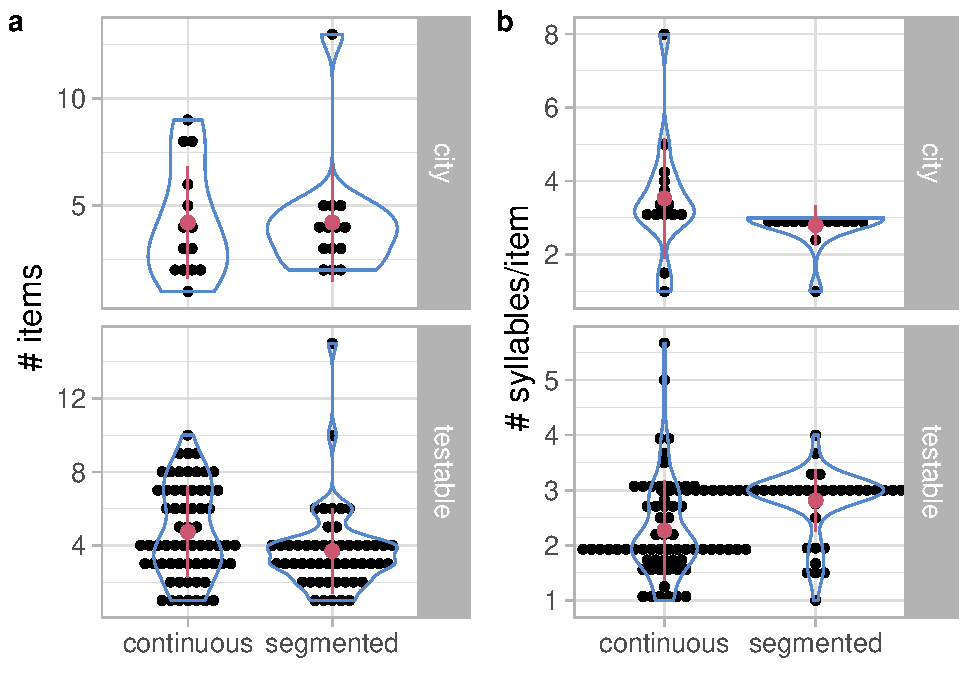
\includegraphics[width=0.8\linewidth]{segmentation_recall_combined_files/figure-latex/recall-general-measures-plot-1} 

}

\caption{Number of items produced as well as their numbers of syllables.}\label{fig:recall-general-measures-plot}
\end{figure}

\subsection{Word vs.~part-word
analysis}\label{word-vs.part-word-analysis}

We next calculate the number and proportion of among (productions) of
words and part-words respectively; we also accept concatenations of
words and part-words. The proportions will be compared across stream
types as well as to zero.

Finally, we calculate the proportion of words among the word and
part-word productions. This proportion will be compared across
segmentation types, as well as to the chance level of 50\%.

As shown in Table \ref{tab:recall-general-results-print} and in Figure
\ref{fig:recall-words-part-words-plot}, participants produced a positive
number of words only in the segmented condition, but not in the
continuous condition. In contrast, they produced a positive number of
part-words only in the continuous condition, but not in the segmented
condition. Accordingly, the proportion of words among words and
part-words was significantly greater than 50\% in the segmented
condition, but numerically (though not significantly) smaller than 50\%
in the continuous condition. The latter result is consistent with
participants randomly picking a syllable to start their vocalizations;
if so, part-words should be 2 times as likely as words.

\begin{figure}

{\centering 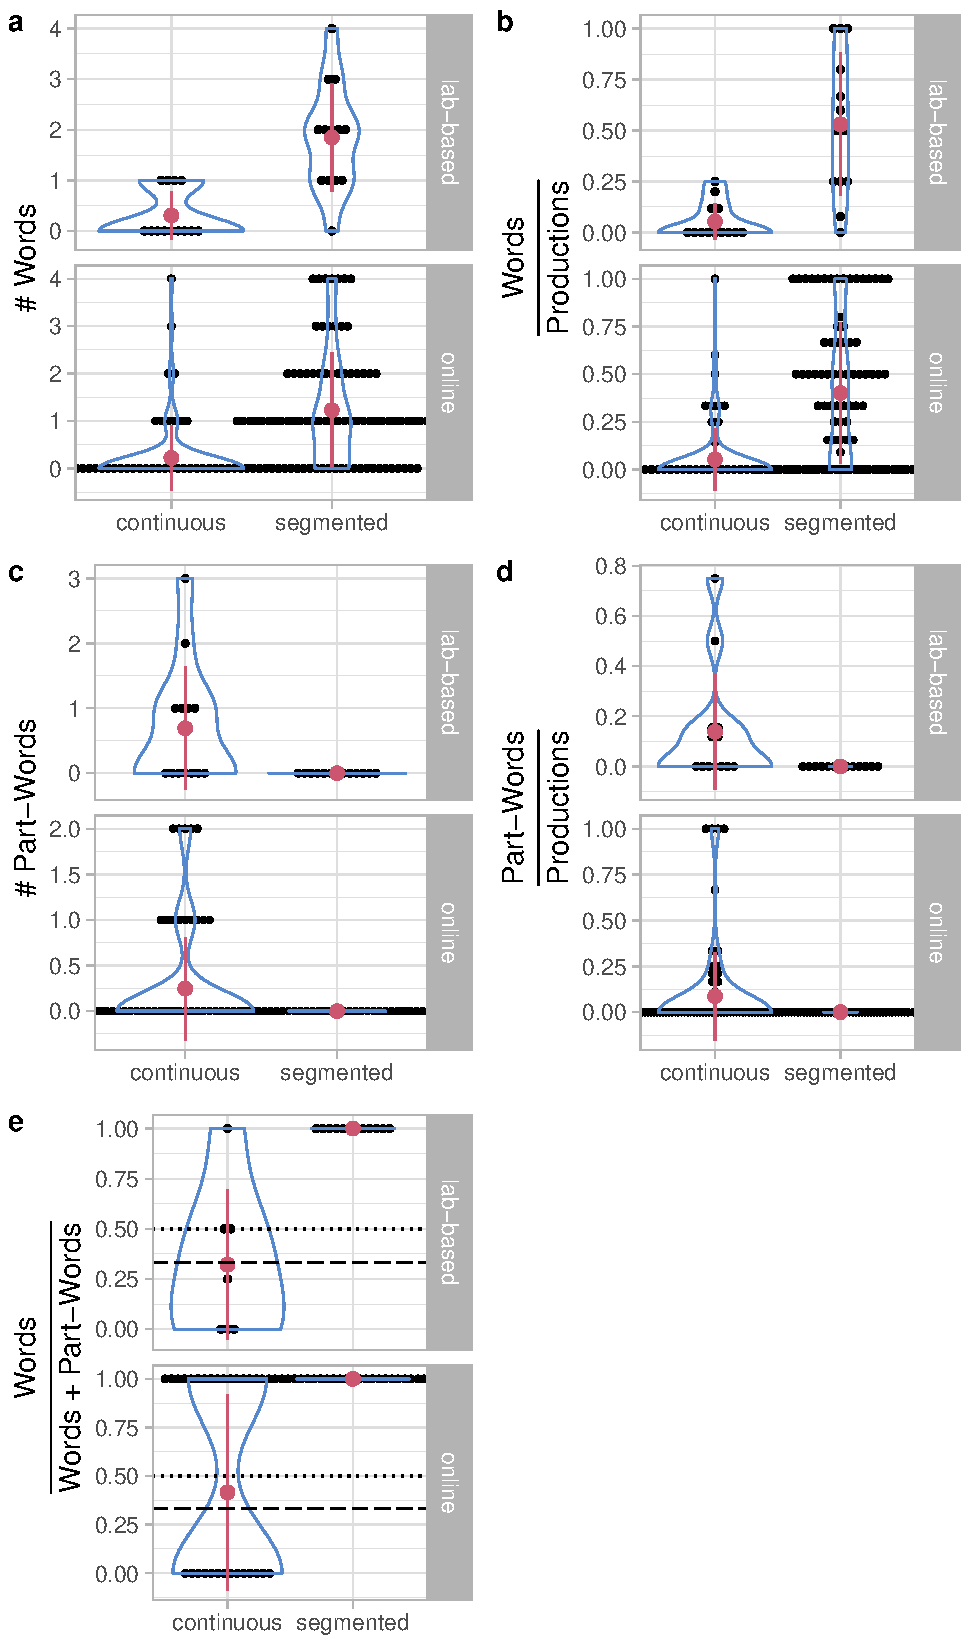
\includegraphics[width=0.8\linewidth]{segmentation_recall_combined_files/figure-latex/recall-words-part-words-plot-1} 

}

\caption{Plot of various comparisons between words and part-words.}\label{fig:recall-words-part-words-plot}
\end{figure}

\subsection{TP-based analyses}\label{tp-based-analyses}

We first computed the average forward TPs in the produced items, and
separately for each segmentation condition, compared it to both the
expected TPs for random strings and the expected TPs given the starting
syllable.

\begin{itemize}
\tightlist
\item
  The expected TPs for items of at least 2 syllables starting on an
  initial syllable are c(1, 1/3, 1, 1, 1/3, 1, 1, 1/3, \ldots{}). The
  difference between the actual and the expected TP needs to be compared
  to zero, as the expected TP differs across items.
\item
  The expected TPs for a random concatenation are the TPs in a random
  bigram. For an A or a B syllable, the random TP is 1 \(\times\) 1 /
  12, as there is only 1 (out of 12) non-zero TP continuations. For a C
  syllable, the random TP is 3 \(\times\) 1/3 / 12, as there are 3
  possible concatenations. On average, the random TP is thus
  \((1/12 + 1/12 + 1/12)/ 3 = 1/12 \approx .083\).
\end{itemize}

We compared these measures across segmentation conditions.

As shown in Table \ref{tab:recall-general-results-print} and Figure
\ref{fig:recall-tps-plot}, forward and backward TPs were significantly
greater than expected for a random string in both the continuous and the
segmented condition, with greater TPs in the segmented conditions.
However, they were significantly \emph{lower} than the TPs expected if
items recalled faithfully, given their starting position.

As shown in Figure \ref{fig:recall-tp-chunks-plot}, participants
produced a positive number of high-TP chunks in both the segmented and
the continuous condition, with a significantly greater number in the
segmented condition. In contrast, they produced a positive number of
low-TP chunks only in the continuous condition. Accordingly, the
proportion of high-TP chunks among high- and low-TP chunks exceeded 50\%
only in the segmented condition.

\begin{figure}

{\centering 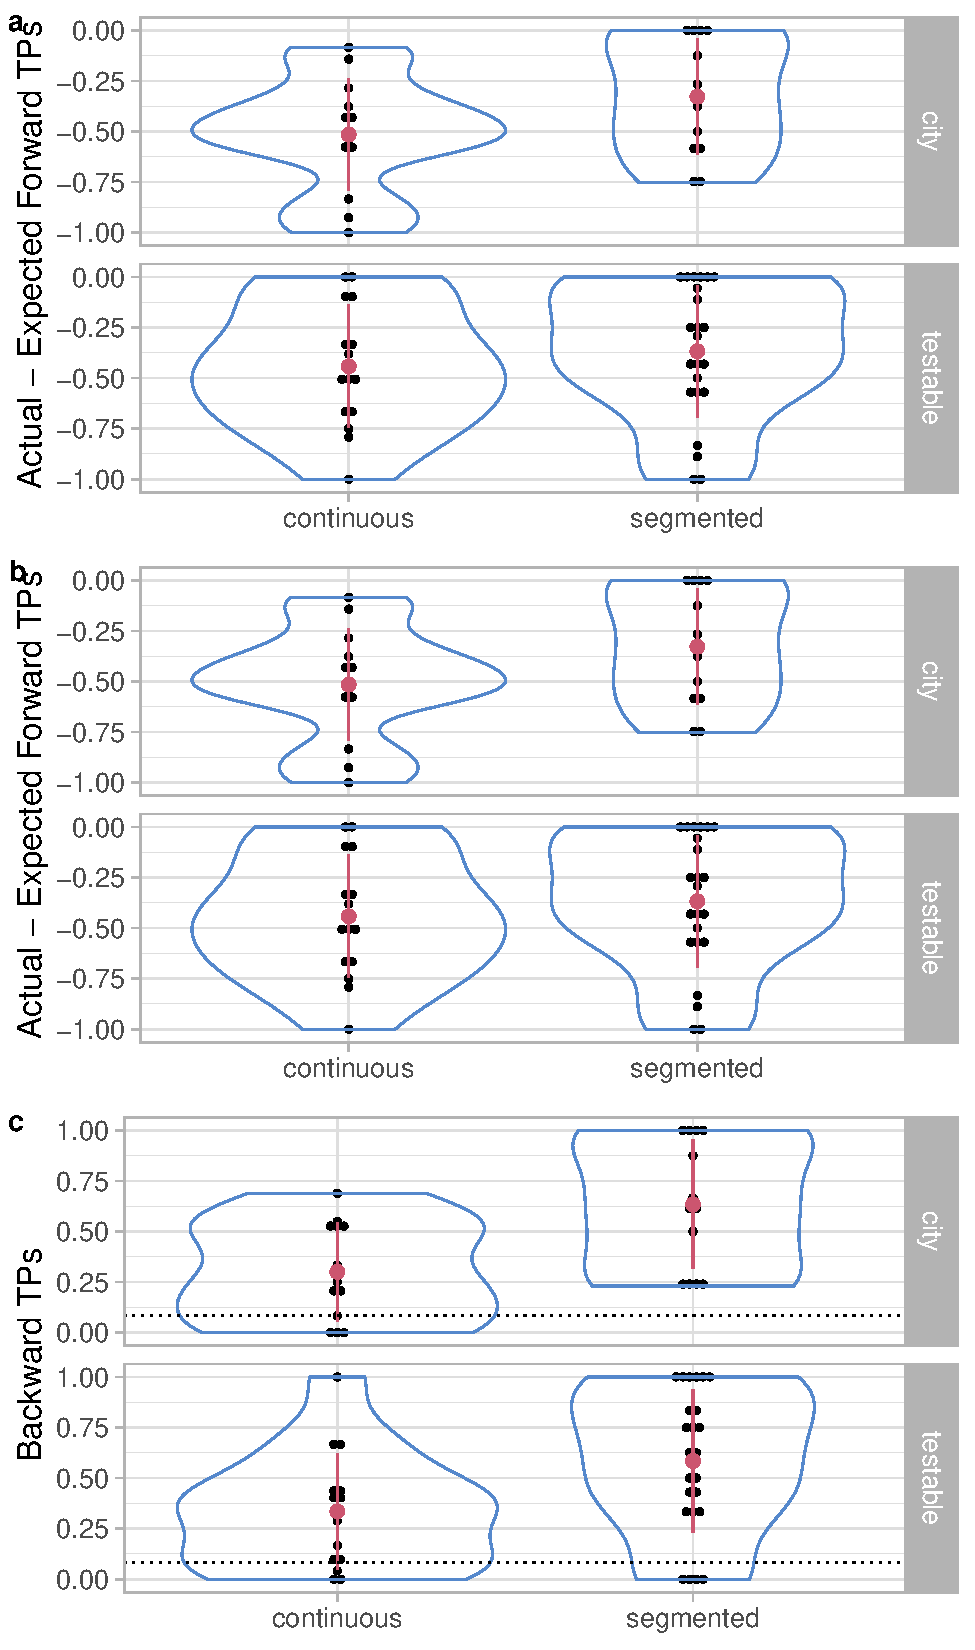
\includegraphics[width=0.8\linewidth]{segmentation_recall_combined_files/figure-latex/recall-tps-plot-1} 

}

\caption{Plot of TP comparisons.}\label{fig:recall-tps-plot}
\end{figure}

\begin{figure}

{\centering 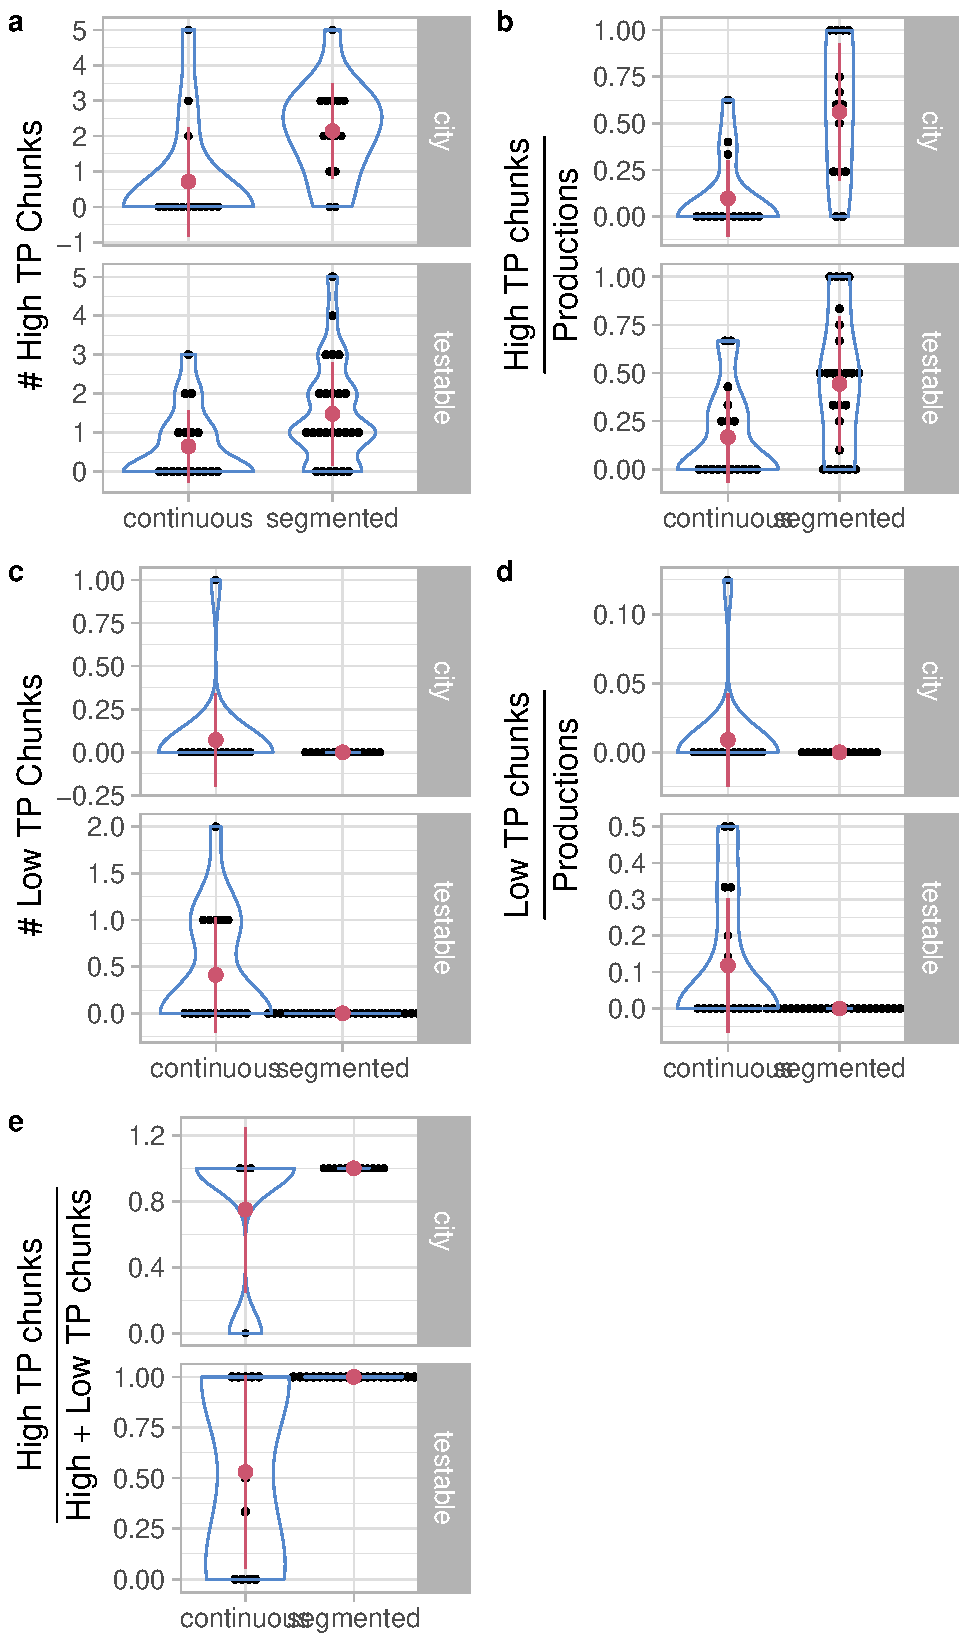
\includegraphics[width=0.8\linewidth]{segmentation_recall_combined_files/figure-latex/recall-tp-chunks-plot-1} 

}

\caption{Plot of High and Low TP chunks.}\label{fig:recall-tp-chunks-plot}
\end{figure}

\subsection{Positional analyses}\label{positional-analyses}

Finally, we analyze the productions in terms of correct initial final
positions. As there are four initial and final positions, respectively,
4/12 of the productions should have ``correct'' initial positions, 4/12
should have correct final positions, while
\(2 \times 4/12 - (4/12)^2 = 5/9\) should have either correct initial or
final positions.

As shown in Table \ref{tab:recall-general-results-print} and Figure
\ref{fig:recall-positions-plot}, participants produced items with
correct initial or final positions at great than chance level only in
the segmented condition, but not the continuous condition.

\begin{figure}

{\centering 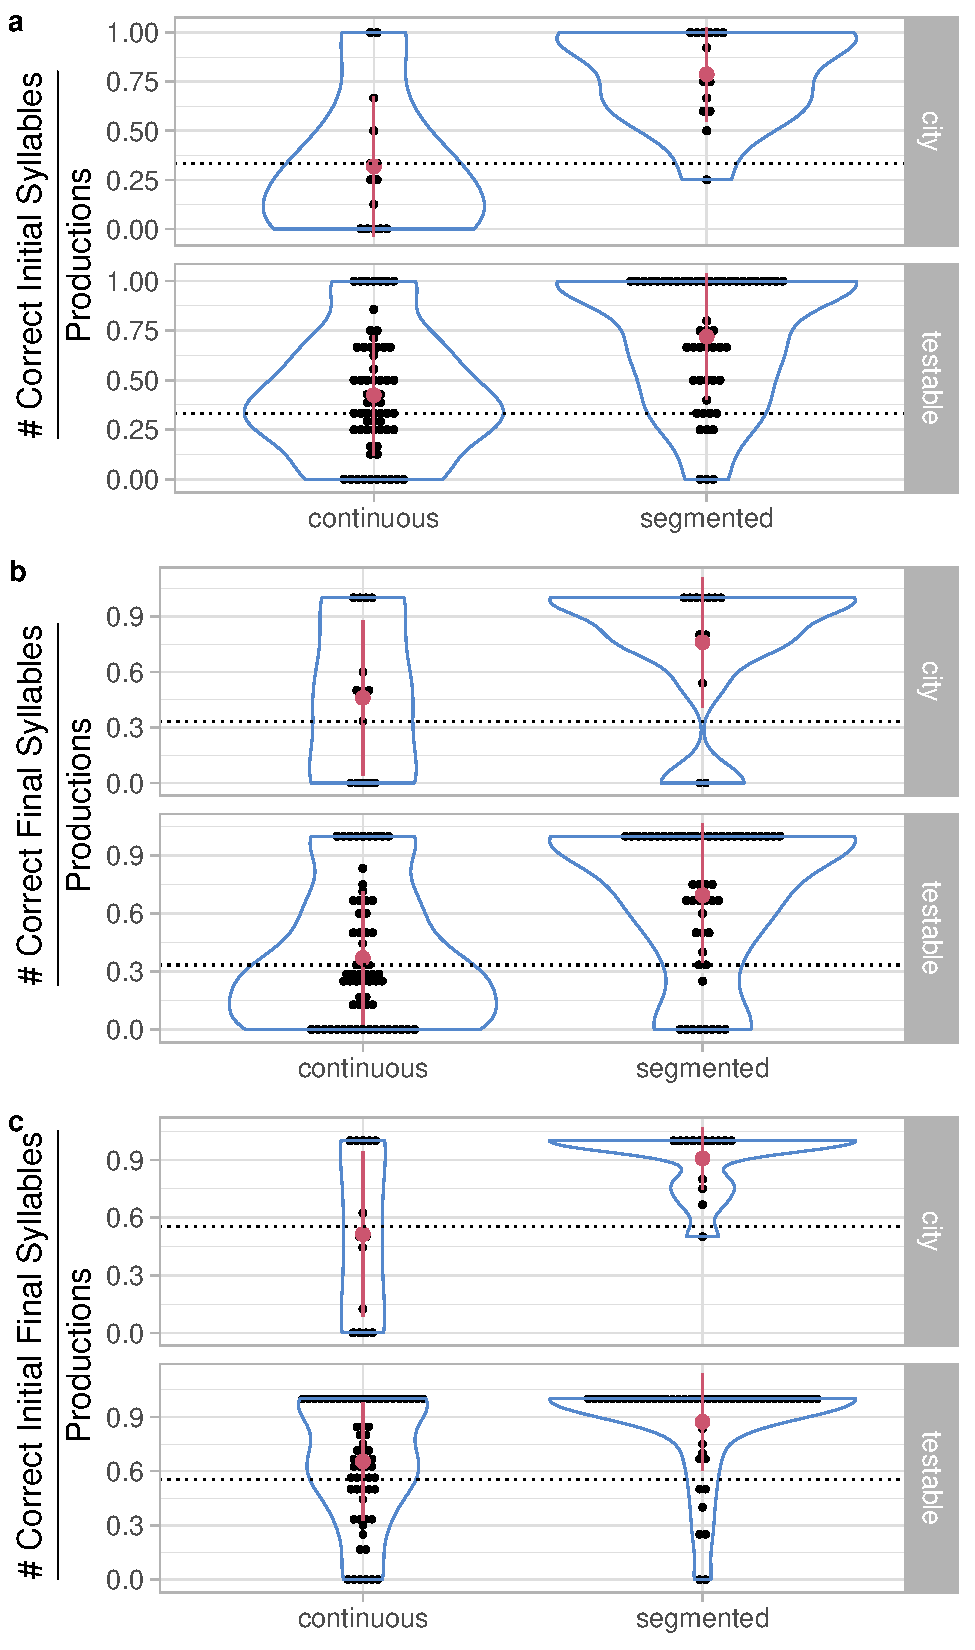
\includegraphics[width=0.8\linewidth]{segmentation_recall_combined_files/figure-latex/recall-positions-plot-1} 

}

\caption{Plot of chunks with correct initial or final positions.}\label{fig:recall-positions-plot}
\end{figure}

\textbackslash{}begin\{table\}

\textbackslash{}caption\{\label{tab:recall-general-results-print}Various
analyses pertaining to the productions as well as test against their
chances levels. Number of items produced, their numbers of syllables,
number of words, number of part-words (chance level: 0), proportion of
words among productions, proportion of part-words among productions,
proportion of words among words and part-words (chance level 50\%),
average forward TPs (chance level: 1/12), difference between
positionally expected and actual TPs, average backward TPS. CHUNKS \}
\centering

\begin{tabular}[t]{llr}
\toprule
Continuous & Segmented & $p_{cont vs. segm}$\\
\midrule
\addlinespace[0.3em]
\multicolumn{3}{l}{\textbf{Number of items}}\\
\hspace{1em}\M = 3.97, \SE = 0.415, \p = 1.14e-06 & \M = 3.77, \SE = 0.366, \p = 4.58e-08 & 0.800\\
\addlinespace[0.3em]
\multicolumn{3}{l}{\textbf{Number of syllables/item}}\\
\hspace{1em}\M = 2.78, \SE = 0.274, \p = 1.15e-06 & \M = 2.71, \SE = 0.0966, \p = 1.03e-08 & 0.667\\
\addlinespace[0.3em]
\multicolumn{3}{l}{\textbf{Number of words}}\\
\hspace{1em}\M = 0.129, \SE = 0.0622, \p = 0.0719 & \M = 1.41, \SE = 0.196, \p = 1.92e-06 & \vphantom{1} 0.000\\
\addlinespace[0.3em]
\multicolumn{3}{l}{\textbf{Proportion of words among vocalizations}}\\
\hspace{1em}\M = 0.129, \SE = 0.0622, \p = 0.0719 & \M = 1.41, \SE = 0.196, \p = 1.92e-06 & 0.000\\
\addlinespace[0.3em]
\multicolumn{3}{l}{\textbf{Number of part-words}}\\
\hspace{1em}\M = 0.323, \SE = 0.128, \p = 0.0179 & \M = 0, \SE = 0, \p = NaN & \vphantom{1} 0.002\\
\addlinespace[0.3em]
\multicolumn{3}{l}{\textbf{Proportion of part-words among vocalizations}}\\
\hspace{1em}\M = 0.323, \SE = 0.128, \p = 0.0179 & \M = 0, \SE = 0, \p = NaN & 0.002\\
\addlinespace[0.3em]
\multicolumn{3}{l}{\textbf{Proportion of part-words among words and part-words}}\\
\hspace{1em}\M = 0.281, \SE = 0.138, \p = 0.182 & \M = 1, \SE = 0, \p = 7.75e-08 & 0.000\\
\addlinespace[0.3em]
\multicolumn{3}{l}{\textbf{Forward TPs}}\\
\hspace{1em}\M = 0.32, \SE = 0.0506, \p = 0.000215 & \M = 0.602, \SE = 0.0563, \p = 2.49e-07 & \vphantom{1} 0.001\\
\addlinespace[0.3em]
\multicolumn{3}{l}{\textbf{Actual vs. Expected Forward TPs}}\\
\hspace{1em}\M = -0.476, \SE = 0.0557, \p = 8.77e-06 & \M = -0.353, \SE = 0.0517, \p = 5.88e-06 & 0.083\\
\addlinespace[0.3em]
\multicolumn{3}{l}{\textbf{Backward TPs}}\\
\hspace{1em}\M = 0.32, \SE = 0.0506, \p = 0.000215 & \M = 0.602, \SE = 0.0563, \p = 2.49e-07 & 0.001\\
\addlinespace[0.3em]
\multicolumn{3}{l}{\textbf{Number of High TP chunks}}\\
\hspace{1em}\M = 0.677, \SE = 0.223, \p = 0.00545 & \M = 1.72, \SE = 0.22, \p = 9.56e-07 & 0.000\\
\addlinespace[0.3em]
\multicolumn{3}{l}{\textbf{Proportion of High TP chunks among productions}}\\
\hspace{1em}\M = 0.136, \SE = 0.0403, \p = 0.00573 & \M = 0.486, \SE = 0.0577, \p = 1.11e-06 & 0.000\\
\addlinespace[0.3em]
\multicolumn{3}{l}{\textbf{Number of Low TP chunks}}\\
\hspace{1em}\M = 0.258, \SE = 0.0939, \p = 0.0147 & \M = 0, \SE = 0, \p = NaN & 0.002\\
\addlinespace[0.3em]
\multicolumn{3}{l}{\textbf{Number of Low TP chunks among productions}}\\
\hspace{1em}\M = 0.0689, \SE = 0.0269, \p = 0.022 & \M = 0, \SE = 0, \p = NaN & 0.002\\
\addlinespace[0.3em]
\multicolumn{3}{l}{\textbf{Proportion of High TP chunks among High and Low TP chunks}}\\
\hspace{1em}\M = 0.589, \SE = 0.127, \p = 0.446 & \M = 1, \SE = 0, \p = 2.75e-08 & 0.000\\
\addlinespace[0.3em]
\multicolumn{3}{l}{\textbf{Proportion of items with correct initial syllables}}\\
\hspace{1em}\M = 0.356, \SE = 0.0602, \p = 1 & \M = 0.753, \SE = 0.0471, \p = 5.07e-07 & 0.000\\
\addlinespace[0.3em]
\multicolumn{3}{l}{\textbf{Proportion of items with correct final syllables}}\\
\hspace{1em}\M = 0.495, \SE = 0.0716, \p = 0.0573 & \M = 0.749, \SE = 0.0542, \p = 8.03e-07 & 0.006\\
\addlinespace[0.3em]
\multicolumn{3}{l}{\textbf{Proportion of items with correct initial or final syllables}}\\
\hspace{1em}\M = 0.622, \SE = 0.0715, \p = 0.482 & \M = 0.906, \SE = 0.0336, \p = 2.76e-07 & 0.001\\
\bottomrule
\end{tabular}

\textbackslash{}end\{table\}

\end{document}
